\subsection{HTTP protokol}
HTTP protokollen er valgt som kommunikations led. 

Der er begrænsede muligheder med 3G/GPS modulet når det kommer til kommunikation. 
Da 3G/GPS modulet ikke understøtter alle kommunikations lag, men understøtter HTTP protokollen er denne protokol valgt som kommunikations lag.
Protokollen understøttes af 3G/GPS modulet, hvilket er den primære årsag til at HTTP protokollen blev valgt som kommunikations lag. 

Derudover er HTTP protokollen den mest anvende protokol til kommunikation mellem en webapplikation og server.
 
HTTP protokol version 1.1 er valgt fremfor 1.0, da version 1.1 indeholder metoden PUT, som er en vigtig metode for systemet.

Metoderne der anvendes er GET, PUT og POST. Når en af disse metoder anvendes, kommer der et svar retur, som indeholder en række informationer.
Svaret indeholder en header og en body, som vist på figur \ref{fig:headerbodyget}. 

Headeren indeholder informationer om HTTP forbindelsen. Den første linje indeholder en status besked, som viser hvorvidt beskeden er blevet modtaget korrekt eller om der er sket en fejl. Ydermere inderholder headeren tidspunktet for modtagelsen, hvilket format body'en er i, tilladte metoder til kommunikation og hvilken type server der er hentet fra. Selve body'en starter på figur \ref{fig:headerbodyget} efter 6b og slutter ved 0, hvor 6b er antal karakterer i body'en vist i hexadecimal. Når PUT eller POST anvendes, er det nødvendigt at sende information for headeren med. Derudover er det vigtigt at sende antal karakterer i bodyen med. Ved PUT og POST modtages der også et svar i form af en header og en body, med de samme informationer som ved GET metoden. 
\begin{figure}[H]
	\centering
	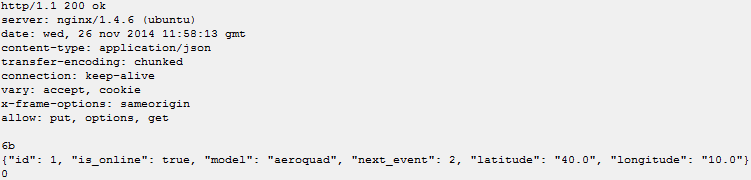
\includegraphics[width=1\textwidth]{Billeder/header_body_get.png}
	\caption{Header og Body for GET metoden}
	\label{fig:headerbodyget}
\end{figure}